% Importado desde: 2026-03-28_Perturbaciones_Dirac_Weyl_3D.tex
\chapter{Perturbaciones Paso a Paso: --- Como un punto de Dirac 3D se gappea o se separa en nodos de Weyl}
\label{ch:perturbaciones-dirac-weyl-3d}






% verified-by: validators/estabilidad_dirac.py::test_mass_anticommutes_kinetic
% verified-by: validators/estabilidad_dirac.py::test_dirac_squared
% verified-by: validators/estabilidad_dirac.py::test_dirac_gap_at_p_zero
% verified-by: validators/estabilidad_dirac.py::test_weyl_no_mass

\section{Objetivo}

En el documento anterior vimos que:

\begin{enumerate}[leftmargin=*]
  \item un nodo de Weyl en \(3D\) se describe con un Hamiltoniano \(2\times 2\);
  \item un punto de Dirac en \(3D\) puede interpretarse como dos nodos de Weyl de quiralidad opuesta superpuestos;
  \item una ruptura de simetria puede separar ese punto de Dirac.
\end{enumerate}

Ahora vamos a dar el paso siguiente con mas detalle: introducir perturbaciones concretas y seguir, calculo a calculo, que le pasa al espectro.

Los tres casos clave seran:

\begin{enumerate}[leftmargin=*]
  \item una \textbf{masa} que abre un gap;
  \item una perturbacion \textbf{separadora} que desdobla el punto de Dirac en dos nodos de Weyl;
  \item la \textbf{competencia} entre ambas, que produce una transicion entre fase gapped y fase Weyl.
\end{enumerate}

\section{Hamiltoniano base de Dirac en 3D}

\subsection{Dos espacios internos}

Para describir un punto de Dirac en \(3D\) necesitamos dos juegos de matrices de Pauli:

\begin{enumerate}[leftmargin=*]
  \item \(\sigma_i\), que actuaran sobre un sector tipo pseudospin;
  \item \(\tau_i\), que distinguiran los dos sectores de Weyl superpuestos.
\end{enumerate}

Un Hamiltoniano minimo y muy util es
\begin{equation}
H_D(\vq)=v\,\tau_z(\sigma_x q_x+\sigma_y q_y+\sigma_z q_z).
\label{c13:eq:HD}
\end{equation}

Este Hamiltoniano puede escribirse tambien como
\begin{equation}
H_D(\vq)=v\,\tau_z\, \vsigma\cdot \vq.
\end{equation}

\subsection{Espectro sin perturbaciones}

Como \((\vsigma\cdot\vq)^2 = q^2 I\), tenemos
\begin{equation}
H_D^2 = v^2 q^2 I,
\qquad
q^2=q_x^2+q_y^2+q_z^2.
\end{equation}

Por tanto,
\begin{equation}
E_\pm(\vq)=\pm v|\vq|,
\label{c13:eq:dirac-disp}
\end{equation}
con degeneracion doble.

Interpretacion:

\begin{enumerate}[leftmargin=*]
  \item la banda superior y la inferior se tocan en \(\vq=0\);
  \item el contacto es lineal en las tres direcciones;
  \item la degeneracion doble refleja que el punto de Dirac contiene dos sectores de Weyl superpuestos.
\end{enumerate}

\begin{figure}[ht]
\centering
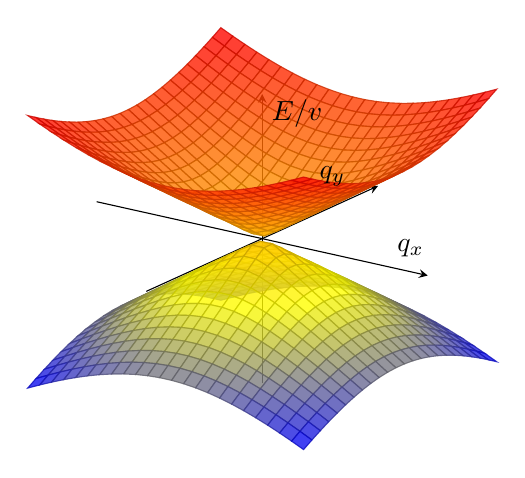
\begin{tikzpicture}
\begin{axis}[
  width=0.72\textwidth,
  view={35}{24},
  axis lines=center,
  xlabel={$q_x$},
  ylabel={$q_y$},
  zlabel={$E/v$},
  xmin=-1.2,xmax=1.2,
  ymin=-1.2,ymax=1.2,
  zmin=-1.5,zmax=1.5,
  ticks=none,
  samples=24,
  domain=-1:1,
  y domain=-1:1
]
\addplot3[surf,opacity=0.8] {sqrt(x^2+y^2)};
\addplot3[surf,opacity=0.8] {-sqrt(x^2+y^2)};
\end{axis}
\end{tikzpicture}
\caption{Corte esquematico del punto de Dirac sin perturbaciones. La linealidad del espectro refleja el comportamiento relativista efectivo.}
\label{c13:fig:dirac-clean}
\end{figure}

\section{Perturbacion 1: termino de masa}

\subsection{Hamiltoniano con masa}

Introducimos ahora
\begin{equation}
H_m(\vq)=v\,\tau_z \vsigma\cdot\vq + m\,\tau_x.
\label{c13:eq:Hmass}
\end{equation}

El punto central es que \(\tau_x\) anticonmuta con \(\tau_z\):
\begin{equation}
\{\tau_x,\tau_z\}=0.
\end{equation}

Como \(\tau_x\) conmuta con las \(\sigma_i\), se sigue que
\begin{equation}
\{\,m\tau_x,\; v\tau_z \sigma_i q_i\,\}=0.
\end{equation}

\subsection{Calculo del espectro}

Elevamos \eqref{c13:eq:Hmass} al cuadrado:
\begin{align}
H_m^2
&=
\left(v\tau_z \vsigma\cdot\vq + m\tau_x\right)^2
\nonumber\\[4pt]
&=
v^2(\tau_z \vsigma\cdot\vq)^2
+ m^2\tau_x^2
+ vm\left[\tau_z \vsigma\cdot\vq\,\tau_x + \tau_x \tau_z \vsigma\cdot\vq\right].
\end{align}

Ahora:

\begin{enumerate}[leftmargin=*]
  \item \(\tau_z^2=I\),
  \item \(\tau_x^2=I\),
  \item \((\vsigma\cdot\vq)^2=q^2 I\),
  \item el termino cruzado se anula por anticonmutacion.
\end{enumerate}

Entonces
\begin{equation}
H_m^2=(v^2 q^2 + m^2)I.
\end{equation}

Por tanto, los autovalores son
\begin{equation}
E_\pm(\vq)=\pm \sqrt{v^2 q^2 + m^2}.
\label{c13:eq:mass-spectrum}
\end{equation}

\subsection{Que significa}

La masa abre un gap de energia
\begin{equation}
\Delta = 2|m|.
\end{equation}

Antes, en \(\vq=0\), las bandas se tocaban en \(E=0\). Ahora:
\begin{equation}
E_\pm(0)=\pm |m|.
\end{equation}

Es decir:

\begin{enumerate}[leftmargin=*]
  \item el punto de Dirac desaparece como cruce gapless;
  \item el sistema pasa a estar gapped;
  \item el termino de masa mezcla los dos sectores de Weyl y los ``pega'' en un estado masivo.
\end{enumerate}

\begin{figure}[ht]
\centering
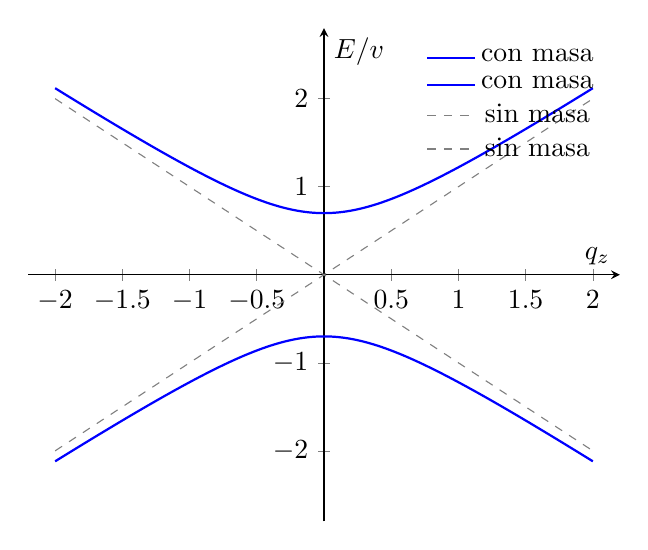
\begin{tikzpicture}
\begin{axis}[
  width=0.75\textwidth,
  xlabel={$q_z$},
  ylabel={$E/v$},
  xmin=-2.2,xmax=2.2,
  ymin=-2.8,ymax=2.8,
  axis lines=middle,
  samples=200,
  domain=-2:2,
  legend style={draw=none,fill=none,at={(0.98,0.98)},anchor=north east}
]
\addplot[thick,blue] {sqrt(x^2+0.7^2)};
\addplot[thick,blue] {-sqrt(x^2+0.7^2)};
\addplot[dashed,gray] {x};
\addplot[dashed,gray] {-x};
\legend{con masa,con masa,sin masa,sin masa}
\end{axis}
\end{tikzpicture}
\caption{Corte unidimensional del espectro. Las curvas grises muestran el caso sin masa; las azules muestran la apertura del gap cuando \(m\neq 0\).}
\label{c13:fig:mass-gap}
\end{figure}

\section{Perturbacion 2: termino que separa nodos}

\subsection{La perturbacion}

Ahora agregamos un termino distinto:
\begin{equation}
H_b(\vq)=v\,\tau_z \vsigma\cdot\vq + b\,\sigma_z.
\label{c13:eq:Hb}
\end{equation}

Este termino no mezcla los dos sectores de Weyl de la misma manera que la masa. En cambio, favorece la direccion \(z\) y termina desplazando los nodos a lo largo de \(q_z\).

\subsection{Calculo usando el cuadrado de H\_b}

Elevamos al cuadrado:
\begin{align}
H_b^2
&=
\left(v\tau_z \vsigma\cdot\vq + b\sigma_z\right)^2
\nonumber\\
&=
v^2 q^2 + b^2 + vb\left(\tau_z \vsigma\cdot\vq\,\sigma_z + \sigma_z \tau_z \vsigma\cdot\vq\right).
\end{align}

Separando componentes:
\begin{equation}
\vsigma\cdot\vq = \sigma_x q_x + \sigma_y q_y + \sigma_z q_z.
\end{equation}

Como \(\sigma_z\) anticonmuta con \(\sigma_x,\sigma_y\) pero conmuta con \(\sigma_z\), los terminos en \(q_x,q_y\) se cancelan y sobrevive solo el de \(q_z\). El resultado es
\begin{equation}
H_b^2 = \left(v^2 q^2+b^2\right)I + 2vb\,q_z\,\tau_z.
\label{c13:eq:Hb-square}
\end{equation}

Puesto que \(\tau_z\) tiene autovalores \(\pm 1\), obtenemos
\begin{equation}
E_\pm^2 = v^2(q_x^2+q_y^2) + (v q_z \pm b)^2.
\label{c13:eq:split-spectrum-square}
\end{equation}

Por tanto,
\begin{equation}
E(\vq)=\pm \sqrt{v^2(q_x^2+q_y^2) + (v q_z \pm b)^2}.
\label{c13:eq:split-spectrum}
\end{equation}

\subsection{Ubicacion de los nodos}

Para que haya energia cero deben anularse simultaneamente:
\begin{equation}
q_x=0,\qquad q_y=0,\qquad v q_z \pm b = 0.
\end{equation}

Luego los nodos quedan en
\begin{equation}
\vq_\pm = \left(0,0,\pm \frac{b}{v}\right).
\label{c13:eq:weyl-nodes-position}
\end{equation}

Esto es exactamente lo que queriamos mostrar:

\begin{enumerate}[leftmargin=*]
  \item el punto de Dirac original en \(\vq=0\) se separa;
  \item aparecen dos nodos de Weyl de quiralidad opuesta;
  \item la distancia entre ellos en momento es proporcional a \(b\).
\end{enumerate}

\begin{figure}[ht]
\centering
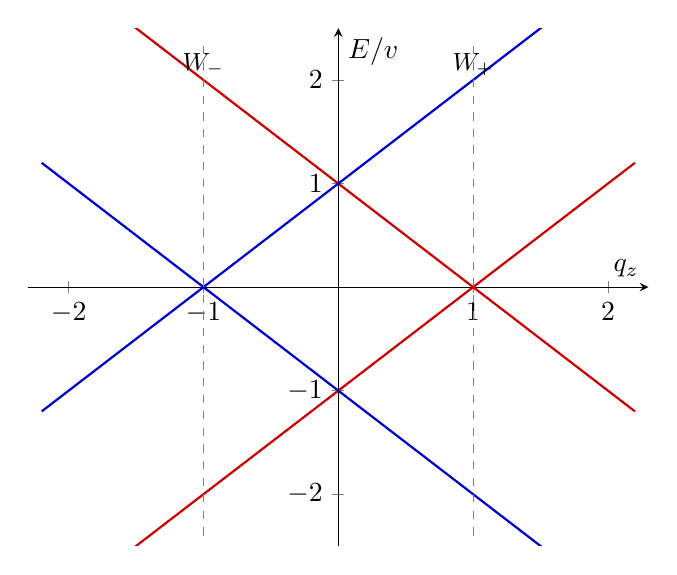
\begin{tikzpicture}
\begin{axis}[
  width=0.78\textwidth,
  xlabel={$q_z$},
  ylabel={$E/v$},
  xmin=-2.3,xmax=2.3,
  ymin=-2.5,ymax=2.5,
  axis lines=middle,
  samples=300,
  domain=-2.2:2.2
]
\addplot[thick,red!80!black] {abs(x-1)};
\addplot[thick,red!80!black] {-abs(x-1)};
\addplot[thick,blue!80!black] {abs(x+1)};
\addplot[thick,blue!80!black] {-abs(x+1)};
\draw[dashed,gray] (axis cs:1,-2.4) -- (axis cs:1,2.4);
\draw[dashed,gray] (axis cs:-1,-2.4) -- (axis cs:-1,2.4);
\node at (axis cs:1,2.15) {\small \(W_+\)};
\node at (axis cs:-1,2.15) {\small \(W_-\)};
\end{axis}
\end{tikzpicture}
\caption{Corte del espectro a lo largo de \(q_z\). El punto de Dirac en el origen se desdobla en dos nodos de Weyl ubicados en \(q_z=\pm b/v\).}
\label{c13:fig:split-qz}
\end{figure}

\section{Perturbacion 3: competencia entre masa y separacion}

\subsection{Hamiltoniano completo}

Ahora ponemos juntos ambos efectos:
\begin{equation}
H(\vq)=v\,\tau_z \vsigma\cdot\vq + m\,\tau_x + b\,\sigma_z.
\label{c13:eq:fullH}
\end{equation}

Este es un modelo muy instructivo porque permite ver una transicion entre:

\begin{enumerate}[leftmargin=*]
  \item una fase gapped;
  \item una fase Weyl.
\end{enumerate}

\subsection{Estrategia}

Para encontrar cuando hay nodos, basta mirar si el sistema puede tener \(E=0\). Para simplificar, buscamos primero posibles nodos sobre el eje \(q_z\), poniendo
\begin{equation}
q_x=q_y=0.
\end{equation}

Entonces
\begin{equation}
H = v q_z \tau_z \sigma_z + m\tau_x + b\sigma_z.
\label{c13:eq:axisH}
\end{equation}

\subsection{Diagonalizacion por bloques}

Como \(\sigma_z\) aparece explicitamente, podemos trabajar en su base. Si \(\sigma_z\) tiene autovalor \(s=\pm 1\), el Hamiltoniano se reduce a una matriz \(2\times 2\) en el espacio \(\tau\):
\begin{equation}
H_s = s\,(v q_z \tau_z + bI) + m\tau_x.
\label{c13:eq:Hs}
\end{equation}

Los autovalores de esta matriz son
\begin{equation}
E_{s,\pm}(q_z)= s\,b \pm \sqrt{v^2 q_z^2 + m^2}.
\label{c13:eq:Es}
\end{equation}

\subsection{Condicion de nodo}

Pedimos \(E=0\):
\begin{equation}
s\,b \pm \sqrt{v^2 q_z^2 + m^2}=0.
\end{equation}

Eso equivale a
\begin{equation}
b^2 = v^2 q_z^2 + m^2.
\end{equation}

Por tanto:

\begin{enumerate}[leftmargin=*]
  \item si \(|b|<|m|\), no hay solucion real para \(q_z\): el sistema esta gapped;
  \item si \(|b|=|m|\), se alcanza el punto critico;
  \item si \(|b|>|m|\), aparecen nodos en
  \begin{equation}
  q_z=\pm \frac{\sqrt{b^2-m^2}}{v}.
  \label{c13:eq:phase-nodes}
  \end{equation}
\end{enumerate}

\subsection{Interpretacion fisica}

La masa intenta unir y gappear los dos sectores de Weyl. El parametro \(b\) intenta separarlos. La fase observada depende de cual de los dos gana.

\begin{figure}[ht]
\centering
\begin{tikzpicture}[scale=1.15,>=Latex]
  \draw[->] (0,0) -- (5.2,0) node[right] {$b$};
  \draw[->] (0,0) -- (0,4.6) node[above] {$m$};

  \draw[thick] (0,0) -- (4.3,4.3);
  \draw[thick] (0,0) -- (4.3,-4.3);

  \fill[blue!12] (0,0) -- (4.3,4.3) -- (0,4.3) -- cycle;
  \fill[orange!15] (0,0) -- (4.3,0) -- (4.3,4.3) -- cycle;

  \node[align=center] at (1.05,2.9) {\small fase gapped\\ \small \(|m|>|b|\)};
  \node[align=center] at (3.15,1.5) {\small fase Weyl\\ \small \(|b|>|m|\)};
  \node[rotate=45,above] at (2.15,2.15) {\small punto critico \(|b|=|m|\)};
\end{tikzpicture}
\caption{Diagrama de fase esquematico en el plano \((b,m)\). La masa abre gap; el parametro \(b\) separa nodos. Cuando \(b\) supera a \(m\), emergen nodos de Weyl.}
\label{c13:fig:phase-diagram}
\end{figure}

\section{Resumen conceptual de los tres casos}

\begin{center}
\begin{tabular}{p{0.22\textwidth}p{0.28\textwidth}p{0.34\textwidth}}
\toprule
\textbf{Perturbacion} & \textbf{Hamiltoniano} & \textbf{Efecto} \\
\midrule
Masa & \(m\tau_x\) & abre gap, \(E=\pm\sqrt{v^2 q^2+m^2}\) \\
Separacion & \(b\sigma_z\) & desplaza nodos a \(q_z=\pm b/v\) \\
Competencia & \(m\tau_x+b\sigma_z\) & fase gapped si \(|m|>|b|\), fase Weyl si \(|b|>|m|\) \\
\bottomrule
\end{tabular}
\end{center}

\section{Mapa visual del argumento}

\begin{figure}[ht]
\centering
\begin{tikzpicture}[
  node distance=8mm and 9mm,
  every node/.style={font=\small},
  box/.style={draw,rounded corners,thick,align=center,minimum width=3.3cm,minimum height=1cm,fill=blue!6},
  arr/.style={-{Latex[length=3mm]},thick}
]
  \node[box] (d) {Dirac 3D\\ \(H_D=v\tau_z\vsigma\cdot\vq\)};
  \node[box, below left=of d] (m) {Agregar masa\\ \(m\tau_x\)};
  \node[box, below right=of d] (b) {Agregar separacion\\ \(b\sigma_z\)};
  \node[box, below=of m] (g) {fase gapped\\ gap \(2|m|\)};
  \node[box, below=of b] (w) {fase Weyl\\ nodos en \(\pm b/v\)};
  \node[box, below right=16mm and -4mm of g] (c) {competencia\\ \(m\tau_x+b\sigma_z\)};

  \draw[arr] (d) -- (m);
  \draw[arr] (d) -- (b);
  \draw[arr] (m) -- (g);
  \draw[arr] (b) -- (w);
  \draw[arr] (g) -- (c);
  \draw[arr] (w) -- (c);
\end{tikzpicture}
\caption{Resumen visual del capitulo.}
\label{c13:fig:roadmap}
\end{figure}

\section{Que queda listo para el siguiente paso}

Con este documento ya quedan claros los mecanismos basicos:

\begin{enumerate}[leftmargin=*]
  \item que termino abre una brecha;
  \item que termino separa nodos;
  \item como aparece una transicion entre fase de Dirac gapped y fase Weyl.
\end{enumerate}

El siguiente paso natural, si seguimos con el mismo estilo, es uno de estos dos:

\begin{enumerate}[leftmargin=*]
  \item derivar de donde salen fisicamente los terminos \(m\tau_x\) y \(b\sigma_z\) a partir de simetrias, inversion y reversibilidad temporal;
  \item introducir campo electromagnetico y derivar de manera pedagogica la idea de anomalia quiral y respuesta de transporte.
\end{enumerate}

Para la secuencia del proyecto, yo seguiria ahora con la opcion 1, porque deja mejor asentado el origen fisico de las perturbaciones antes de pasar a observables.
